% !TEX root = ../thesis.tex
\chapter{Prediction}
\label{capitolo6}
\thispagestyle{empty}
\section{Stacking meta-classifier}
In order to classify bots, we had three models, each with different purposes, but they had to cooperate for the bots' behaviour identification.
The initial idea was to use only the multi-class Random Forest to classify the bot categories, using the other two models as meta-models to build extra features with their outcome.
Those features would have had the dataset enhanced, but their meaning would have been bounded to the multi-class classifier limits.
We wanted to give the right importance to each model, hoping they would help each other to better distinguish the patterns end to better model the real problem.

We thought about several methods to exploit their strengths and combine them. In particular, we thought about a genetic approach and a stacking ensemble with a meta-classifier. 
We wanted to evaluate the performance obtained by these methods and chose the one that fitted our need.

Both the genetic and the meta-model were trained with holdout technique, splitting the whole dataset into training and test sets. The 70\% of the samples ended up into the training set, the 30\% in the validation set.
We had a training set for the ensemble models that contains 6,434 entries.
The data that fed the stacking methods were the predictions of the tree classifiers, over the validation set.
In order to make those prediction without cheating, we couldn't use the models that were already fitted with the hole data. We had to retrain them with the 70\% of the records. 
We didn't perform further Grid Search to find the best hyperparameters in this stage, because the final script that we were going to assemble was taking into account the entire dataset to train the models. Furthermore, this small variation, in terms of amount of training data, wouldn't had led us into a misinterpretation of the problem, if we had kept the same hyperparameters found earlier.
We decided to stick with the configurations already found and to train the model with fewer data.

Once the models were fitted, we used the \textit{predict\_proba()} method of the Scikit-learn implementations of the classifiers, in order to retrieve ``soft classifications``. This method differ from the standard \textit{predict()} function, because it doesn't return the predicted target for that sample, but it returns the computed probabilities for each class. The way a probability is given depends on the classification algorithm, i.e. Random Forest assesses the probability by retrieving the votes that its leaves give to each class. The \textit{predict()} method, instead, after the probability computation, returns the most probable target.
We didn't want our model to assign a strict label to an unseen sample, indeed, we were interested in the percentage of categories membership.
We used this method to construct the output vectors needed to train the stacking models.

Each sample of this new dataset contains 12 elements, 4 soft predictions (one for each category) for each classifier (complete Random Forest, text-based Naive Bayes and user-based KNN).

\begin{center}
	\begin{tabular}{@{}c|c|c|c|c|c|c|c|c|c|c|c@{}}
		\multicolumn{12}{c}{New sample} \\
		\hline
		\multicolumn{4}{c|}{\textbf{KNN prob.}} & 
		\multicolumn{4}{c|}{\textbf{NB prob.}} & 
		\multicolumn{4}{c}{\textbf{RF prob.}}\\
		\hline
		\multicolumn{1}{c|}{p\textsubscript{0}} &
		\multicolumn{1}{c|}{p\textsubscript{1}} &
		\multicolumn{1}{c|}{p\textsubscript{2}} &
		\multicolumn{1}{c|}{p\textsubscript{3}} &
		\multicolumn{1}{c|}{p\textsubscript{4}} &
		\multicolumn{1}{c|}{p\textsubscript{5}} &
		\multicolumn{1}{c|}{p\textsubscript{6}} &
		\multicolumn{1}{c|}{p\textsubscript{7}} &	
		\multicolumn{1}{c|}{p\textsubscript{8}} &
		\multicolumn{1}{c|}{p\textsubscript{9}} &
		\multicolumn{1}{c|}{p\textsubscript{10}} &
		\multicolumn{1}{c}{p\textsubscript{11}}\\
		\hline
	\end{tabular}
\end{center}

A new training set was born and it was built with the soft classifications of the models in the pool, over the validation set. It was ready to proceed and to serve the ensemble models.\\

\begin{figure}[htp!]
	\centering
	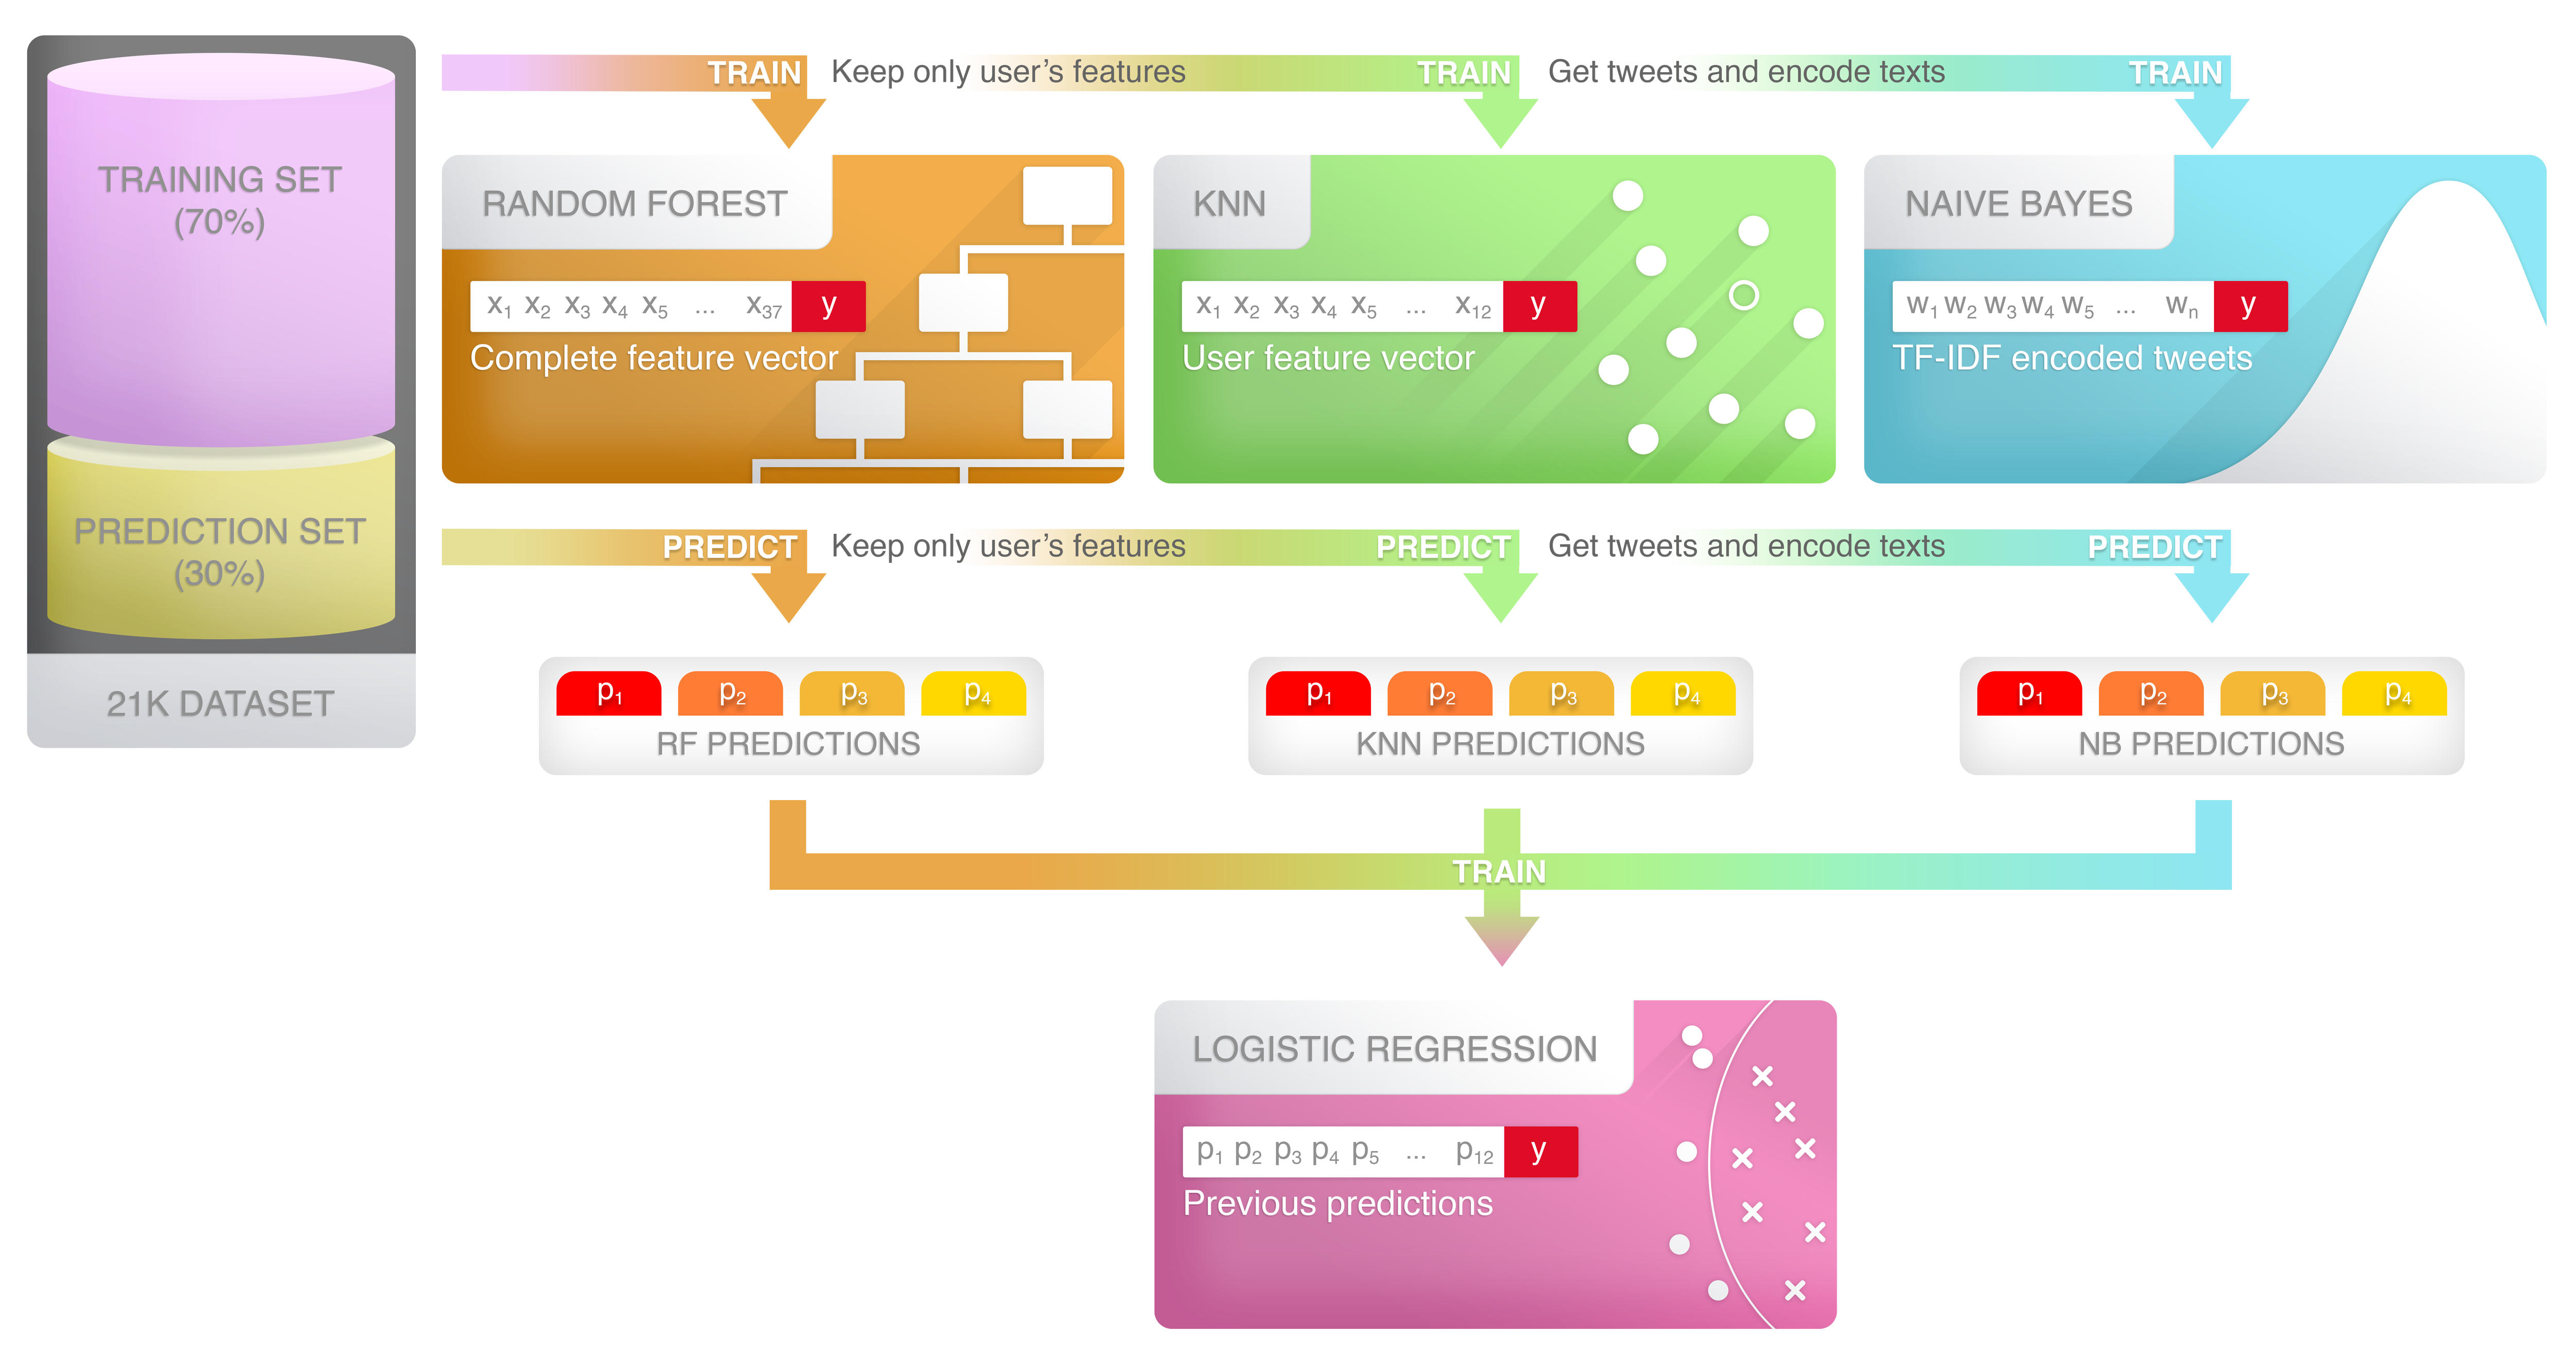
\includegraphics[width=\columnwidth]{chapter5/figure/stacking_train.png}
	\caption{Training pipeline of the stacking ensemble}
	\label{fig:stacking_pipeline}
\end{figure}
The pipeline for perform the training of the ensemble models is resumed in Figure \ref{fig:stacking_pipeline}.

After several parallel attempts were done, the blending system was built with the meta-classifier.

\subsection{Genetic algorithm}
This approach started as a side way, when we were already testing the stacking ensemble.

The idea behind genetic programming, is to emulate the natural species evolution, by encoding the the \textit{chromosomes} in the process with data structures.
The chromosomes represent the possible solutions for the problem and they have to ``evolve``, in order to get fitter and fitter for the goal.
Several operators must be determined to perform this evolution.
Once a first \textit{generation} of feasible chromosomes has been formed, they have to be evaluate according to a \textit{fitness function}, which asses how well a chromosome faces the problem.
The best portion of chromosomes are picked to be part of the next generation, and this is called \textit{elitism}. The solutions left are given a probabilities to join the elite ones, in order to form a new generation with about the same size as the previous. This step is called \textit{selection}.
The chromosomes picked in the selection stage are assigned a high \textit{crossover} probability.
The crossover operator handles the ``born`` of new chromosomes, mixing parents alleles in a certain way. The mixing method is highly correlated to the chosen encoding strategy.
Each newborn is give a low probability to undergo a mutation. This step often seems useless, but it's pretty important, in order to explore a higher spectrum of solutions, which couldn't be expanded by the mating operators only.
After the new population has been accepted, it is ready to be validated through the previously define fitness function.
The loop holds, until a solution is found, or, like in our case, the process sticks to a local or global maximum.

\subsubsection{Genetic operators}

We setted the genetic algorithm with the support of the Deap library for Python, setting these operators:
\begin{itemize}
	\item[\PencilRight]\textit{Encoding}: each chromosomes represented a weighting vector for the outcome of our three classifiers. Each allele of the chromosome was float valued, with numbers between 0 and 5, generated randomly, with a uniform distribution. We started with normalized weights, but the spectrum of the solution explored was way too poor to fit the needs.
	This range was given after observing the weights that the Logistic Regression model were assigning to the inputs received, that was wider and involved even negative values.
	We randomly generated 200 chromosomes for the initial population, with this form.
\end{itemize}
\begin{center}
	\begin{tabular}{@{}c|c|c|c|c|c|c|c|c|c|c|c@{}}
		\multicolumn{12}{c}{Chromosome} \\
		\hline
		\multicolumn{4}{c|}{\textbf{KNN weights}} & 
		\multicolumn{4}{c|}{\textbf{NB weights}} & 
		\multicolumn{4}{c}{\textbf{RF weights}}\\
		\hline
		\multicolumn{1}{c|}{w\textsubscript{0}} &
		\multicolumn{1}{c|}{w\textsubscript{1}} &
		\multicolumn{1}{c|}{w\textsubscript{2}} &
		\multicolumn{1}{c|}{w\textsubscript{3}} &
		\multicolumn{1}{c|}{w\textsubscript{4}} &
		\multicolumn{1}{c|}{w\textsubscript{5}} &
		\multicolumn{1}{c|}{w\textsubscript{6}} &
		\multicolumn{1}{c|}{w\textsubscript{7}} &	
		\multicolumn{1}{c|}{w\textsubscript{8}} &
		\multicolumn{1}{c|}{w\textsubscript{9}} &
		\multicolumn{1}{c|}{w\textsubscript{10}} &
		\multicolumn{1}{c}{w\textsubscript{11}}\\
		\hline
	\end{tabular}
\end{center}
\begin{itemize}
	\item[\PencilRight]\textit{Fitness evaluation}: the fitness function that assessed the value of the solutions was somehow similar to the one used in the other stacking method.
	We applied the weights of our chromosomes to the samples in our dataset.
	
	For each sample, we made pairwise additions, among the outputs of different classifiers, multiplied by the chromosome's weights, for the same category:
	\begin{center}
		\begin{tabular}{@{}c@{}}
			
			\multicolumn{1}{c}{User-based components}\\
			\hline
			\multicolumn{1}{c}{p\textsubscript{0} * w\textsubscript{0} ... p\textsubscript{3} * w\textsubscript{3}}\\
			\hline\\
			\multicolumn{1}{c}{+}\\
			
			\\\multicolumn{1}{c}{Text-based components}\\
			\hline
			\multicolumn{1}{c}{p\textsubscript{0} * w\textsubscript{0} ... p\textsubscript{3} * w\textsubscript{3}}\\
			\hline\\
			\multicolumn{1}{c}{+}\\
			
			\\\multicolumn{1}{c}{All-features-based components}\\
			\hline
			\multicolumn{1}{c}{p\textsubscript{0} * w\textsubscript{0} ... p\textsubscript{3} * w\textsubscript{3}}\\
			\hline\\
			\multicolumn{1}{c}{=}\\
			
			\\\multicolumn{1}{c}{Resulting prediction}\\
			\hline
			\multicolumn{1}{c}{\textbf{p\textsubscript{0}} \textbf{p\textsubscript{1}} \textbf{p\textsubscript{2}} \textbf{p\textsubscript{3}}}\\
			\hline\\
		\end{tabular}
	\end{center}
	
	In order to stick to the probabilities nature, the computed prediction had been normalized.
	
	That prediction has been compared with the known real target for the examined sample.
	Since the targets of our dataset aren't soft valued, we took the maximum probability of the computed prediction to make the comparison with the actual class.
	Our fitness function aims to favourite those solutions which maximizes the F1 macro score, as it has been for the validation of the classifiers, until this stage.
	
	During this process, the problem we had to face was that we wanted to produce soft classifications, because we knew that our collected data presents similar patterns within the same categories. This means that the algorithms easily classify our test set, because of the distinctive traits found for each target. In order to mitigate the real test error, over unseen samples, we wanted the prediction to be as smooth as possible, without confusing the F1 score interpretation.
	
	We faced the problem involving a smoothing factor to our fitness function.\\
	When computing a sample, we populated a Confusion Matrix of the prediction, using the above-mentioned method to match predicted and actual classes. The matrix helped us computing the F1 macro score easily. At the same time, we counted every hard classification, marking as 'hard' every computed prediction that contained a probability greater or equal to \textbf{0.8}, among its five stored values.
	This count was used as a penalty, it has been averaged for the number of samples, and then subtracted to the computed F1 score of that chromosome. In order to privilege the maximization of the F1 factor, instead of the minimization of the penalty, the final fitness function assigned this score to each chromosome:
	\[ Fitness = 3 \times F1\_score - Penalty \]
	This way to operate didn't affect the overall F1 of the sample, since penalizing hard classifications didn't discourage the system to look for values high enough to have a dominant category in the prediction.
	
	Once every chromosome has been evaluated, they could proceed to the next steps of the algorithm.
	
	\item[\PencilRight]\textit{Selection}: the selection phase handles the choice over which chromosomes pick for mating. Several pre-implemented methods are available, but we used the tournament method. It works selecting the size \textit{K} of the tournament, which we chose to be 3. Then, it randomly selects \textit{K} (3) chromosomes from the population and places it inside a pool. Then it compares their fitness. The chromosome with the best fitness has probability \textit{p} (the crossover probability) to be selected for mating. The second has $ p*(1-p) $ chance to get selected, the third $ p*((1-p)^{2}) $.
	\item[\PencilRight]\textit{Crossover}: The crossover probability has been setted to 95\%.
	The crossover operator wasn't something already implemented by the library, as for the fitness function. Our operator used to produce two brand new chromosomes for the next generations.
	The first child is the unweighted mean of its parents:
	\[ [x_{0}, x_{1}, ... x_{11}] \oplus [y_{0}, y_{1}, ... y_{11}] = [\frac{x_{0}+y_{0}}{2}, \frac{x_{1}+y_{1}}{2}, ... \frac{x_{11}+y_{11}}{2}]\]
	The second child is the weighted mean of its parents, computing the weights with respect to the fitness of the two mating chromosomes:
	\[ f_{x} = \frac{fitness_{x}}{fitness_{x}+fitness_{y}} \]
	\[ f_{y} = \frac{fitness_{y}}{fitness_{x}+fitness_{y}} \]
	\[ [x_{0}, x_{1}, ..., x_{11}] \oplus [y_{0}, y_{1}, ..., y_{11}] = [x_{0}*f_{x}+y_{0}*f_{y}, ... x_{11}*f_{x}+y_{11}*f_{y} ]\]
	
	The retrieved children used to be part of the upcoming generation.
	\item[\PencilRight]\textit{Elitism}: This part was necessary, in order to not lose the best solutions found so far. It is a sort of insurance, which guarantees to keep, at least, the best situation until this stage, and to let it take part of the next generations of solution. We preserved our three best chromosomes for each generations and move them to the next stages.
	\item[\PencilRight]\textit{Mutation}: The mutation probability is generally setted to low values, like what happens in nature. It represent the error in DNA replications from the parents and it shouldn't reach the 1\% of probability to occur.
	Although, we wanted to force some mutation, because, as said before, we needed a wider space of solutions and the elitism helped us in containing the damages of such mutations. In the worst cases, all the chromosomes have had been damaged and resulted as useless, but the elitism had preserved the best ones and kept it untouched. So we imposed a 45\% of mutation probability, for each newborn solutions, before entering the pool.
	
	Our mutation operator was a decoration of the value changing method already implemented: we randomly used to pick three elements from the chromosome and set them to zero.
\end{itemize}

\subsubsection{Results}
After several runs of the genetic program, with boosted starts (the best solutions found at the previous run were placed inside the first generations of the following runs), we stuck in a maximum of the score.
In the last run, from the 5\textsubscript{th} generation there was no improvements in the fitness of the best solution. We selected the fittest chromosome, whose scores were:
\begin{itemize}
	\item[\PencilRight] \textit{Weights}:
	
	\begin{center}
		\begin{tabular}{@{}c|c|c|c@{}}
			\hline\hline
			\multicolumn{4}{c}{\textbf{KNN Weights}}\\
			\hline
			\multicolumn{1}{c|}{2.452}&
			\multicolumn{1}{c|}{4.104}&
			\multicolumn{1}{c|}{0.0}&
			\multicolumn{1}{c}{0.0}\\
			\hline
			\multicolumn{4}{c}{\textbf{NB Weights}}\\
			\hline
			\multicolumn{1}{c|}{4.766}&
			\multicolumn{1}{c|}{1.0}&
			\multicolumn{1}{c|}{0.0}&
			\multicolumn{1}{c}{0.0}\\
			\hline
			\multicolumn{4}{c}{\textbf{RF Weights}}\\
			\hline
			\multicolumn{1}{c|}{3.790}&
			\multicolumn{1}{c|}{1.0}&
			\multicolumn{1}{c|}{1.08}&
			\multicolumn{1}{c}{2.506}\\
			\hline\hline
		\end{tabular}
	\end{center}
	\item[\PencilRight] \textit{Fitness}: 0.768
	\item[\PencilRight] \textit{F1 score}: 0.44
	\item[\PencilRight] \textit{Percentage of hard classifications}: 55.3\%
\end{itemize}

The results were discouraging, compared to the singular scores of the models involved.
It was worth to try this approach, but we were aware that a ``simple`` weighted mean of the outcomes of the classifiers weren't enough to describe the problem.

Thus, we built a different and more sophisticated stacking method.

\subsection{Logistic Regression}
The reason behind the choice of a meta-classifier is that we wanted a more complex way to perform inner weighting of the outcomes that we had from other models.
A simple weighted mean wasn't enough for this purpose. Furthermore, implementing a logistic-like loss to evaluate the fitness of a genetic algorithm would have mean to apply the Logistic Regression training model, without performing gradient descent, but with a genetic approach. It would have been just unnecessary and computationally expensive.
Thus, we discarded the idea of using the genetic programming to emulate a Logistic model, even if the smoothing factor used for that try was a good insight for our task.
In order to mitigate the lacking of soft classifications, we chose to rely on the regularization factors that belong to the training algorithm of the Logistic Regression.
This kind of models is often involved in stacking other classifiers, with a binary purpose.

\subsubsection{Dataset}
The same training set has been used for train both the Genetic and Logistic models.
Since we were managing a multi-class datasets, we knew that the ensemble meta-model would had been adapted to this job. The most common tool used for stacking purposes is the Logistic Regression, which performs well on binary separations. We decided to test this model on a multinomial approach, with a softmax activation function, instead of trying the already visited One-vs-Rest method.

\subsubsection{Comparison with Random Forest}
We didn't want to blindly select this model over some others tool, especially over Random Forest, which proved us to perform well in multi-class classifications.
Thus, we tested these two algorithms with the new dataset.
We ran some default configurations of the models, in order to have a raw comparison to trace a line between them.


\begin{figure}[htp!]
	\centering 
	\subfigure[LogReg with raw settings]{
		\label{fig:lr_def}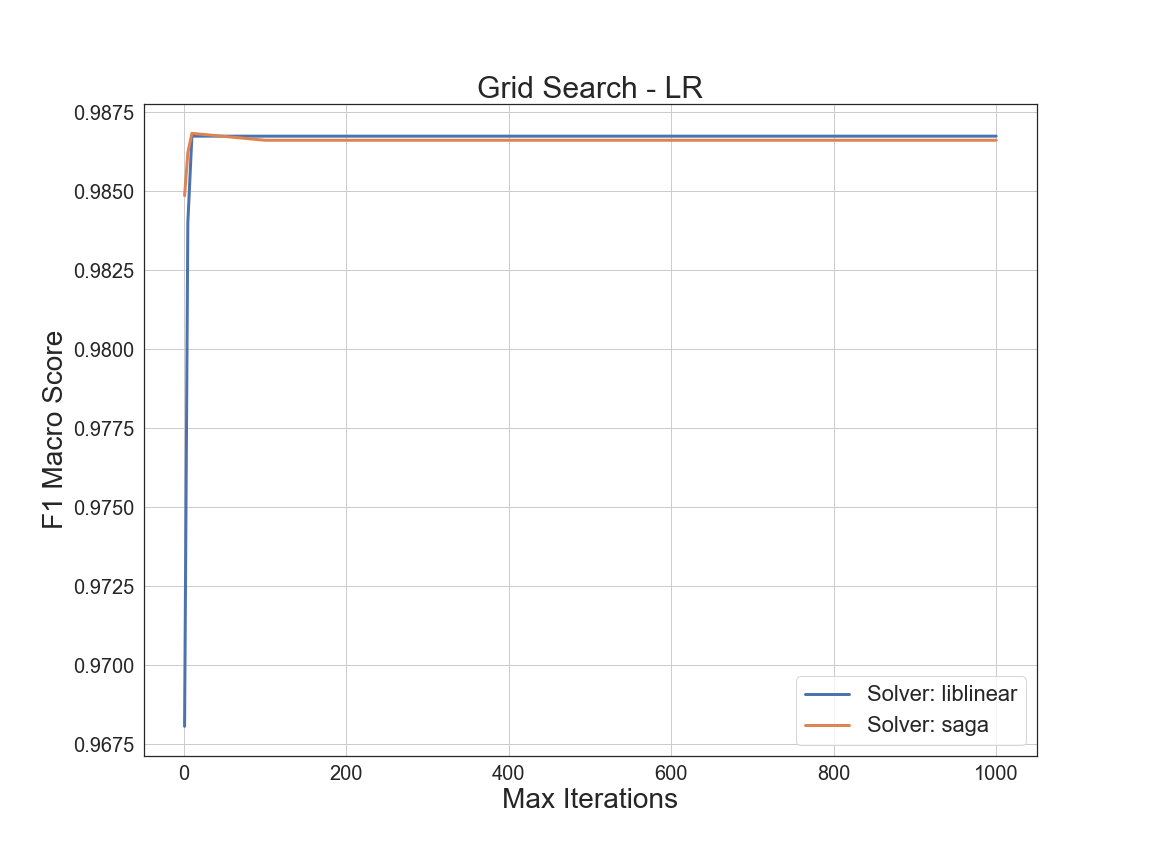
\includegraphics[width=\columnwidth]{chapter5/figure/logreg_default.png}}
	\subfigure[Random Forest with raw settings]{
		\label{fig:rf_def}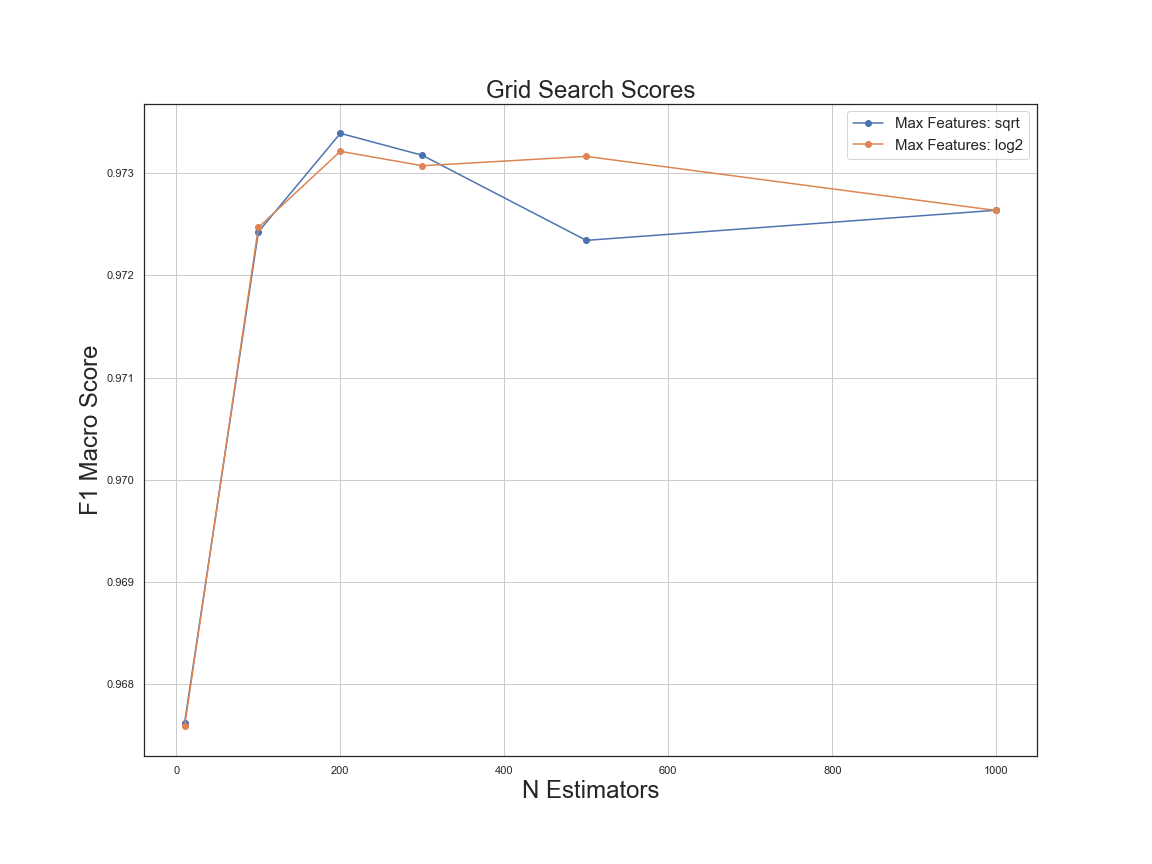
\includegraphics[width=\columnwidth]{chapter5/figure/random_forest_default.png}}
	\caption{Stacking models comparison}
\end{figure}

Figure \ref{fig:lr_def} shows the early convergence of the Logistic model's F1 score, with low maximum iterations. The model has been tested with Lasso penalty and two different solvers, but the results, over the increasing of the training epochs, are way similar.
Although the Random Forest, as shown in Figure \ref{fig:rf_def}, tops the performance of the Logistic Regression, the scores were close enough (F1\textsubscript{LR} = 0.9868,  F1\textsubscript{RF} = 0.9874) to give a chance to the Logistic model, in order to try its regularization terms.

\subsubsection{Hyperparameters tuning}
We tried two regularization terms for the Logistic model and several numbers of maximum iterations for the training algorithms.
The regularization terms are parameters computed in addition with the minimization of the characteristic loss function. Their purpose is to avoid the weights to explode and the model to become more sensitive to noisy data. In other words, they are involved to prevent overfitting.
The idea is that the loss function, gets modified as follows
\[ \mathbf{L(w)} = L_{D}(w) + \lambda L_{W}(w)\]
Where $ L_{D}(w)  $ represent the error on the data and $ L_{W}(w)  $ is the term representing the model complexity. In general, smoother weights implies lower model complexity. The lighter the complexity, the lower the variance of the model and the risk perform overfitting.
The parameter $ \mathit{\lambda} $ has to be tuned with a validation method.

The penalties that we explored were:
\begin{itemize}
	\item[\PencilRight] \textit{Lasso (L\textsubscript{1})}:
	\[ \mathbf{L_{1}(w) }= \frac{\lambda}{2} ||\mathbf{w}||_{1} \]
	where $ ||\mathbf{w}||_{1} = \sum_{i=1}^{N}|w_{i}| $
	
	This regularization function is non-linear and doesn't provide a closed-form solution. It tends to cut out some features from the model, yielding to sparse and lighter model. It can be seen as an implicit way to apply features selection.
	
	\item[\PencilRight] \textit{Ridge (L\textsubscript{2})}:
	\[ \mathbf{L_{2}(w) }= \frac{\lambda}{2} ||\mathbf{w}||^{2}_{2} \]
	where $ ||\mathbf{w}||^{2}_{2} = \sum_{i=1}^{N}w_{i}^{2} $
	
	This softer term tends to shrink the weights, keeping the loss function quadratic in \textbf{w} and closed forum solution exists.
\end{itemize}

\begin{figure}[htp!]
	\centering 
	\subfigure[Lasso penalty, $ \lambda$ = (0.1, 1, 10, 100)]{
		\label{fig:lr_lasso_lambda}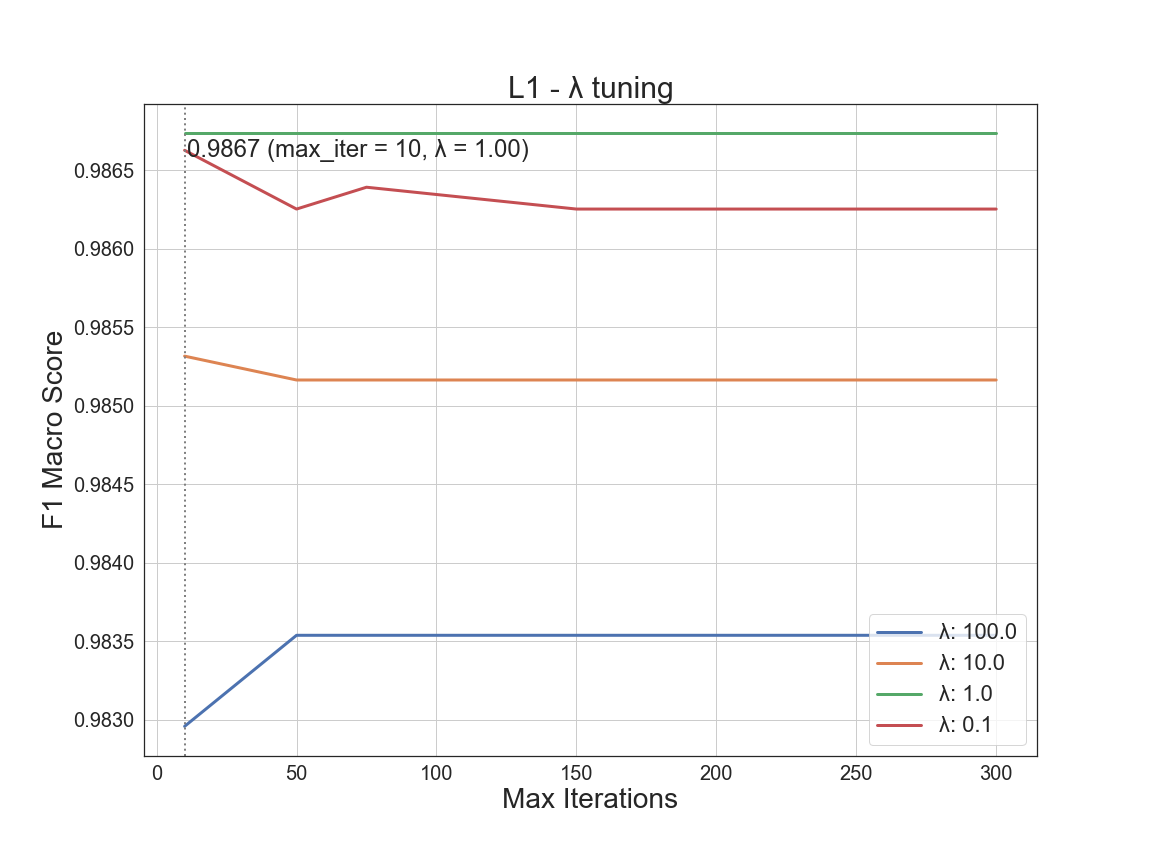
\includegraphics[width=\columnwidth]{chapter5/figure/logreg_l1_lambda.png}}\par 
	\subfigure[Ridge penalty, $ \lambda$ = (0.1, 1, 10, 100)]{
		\label{fig:lr_ridge_lambda}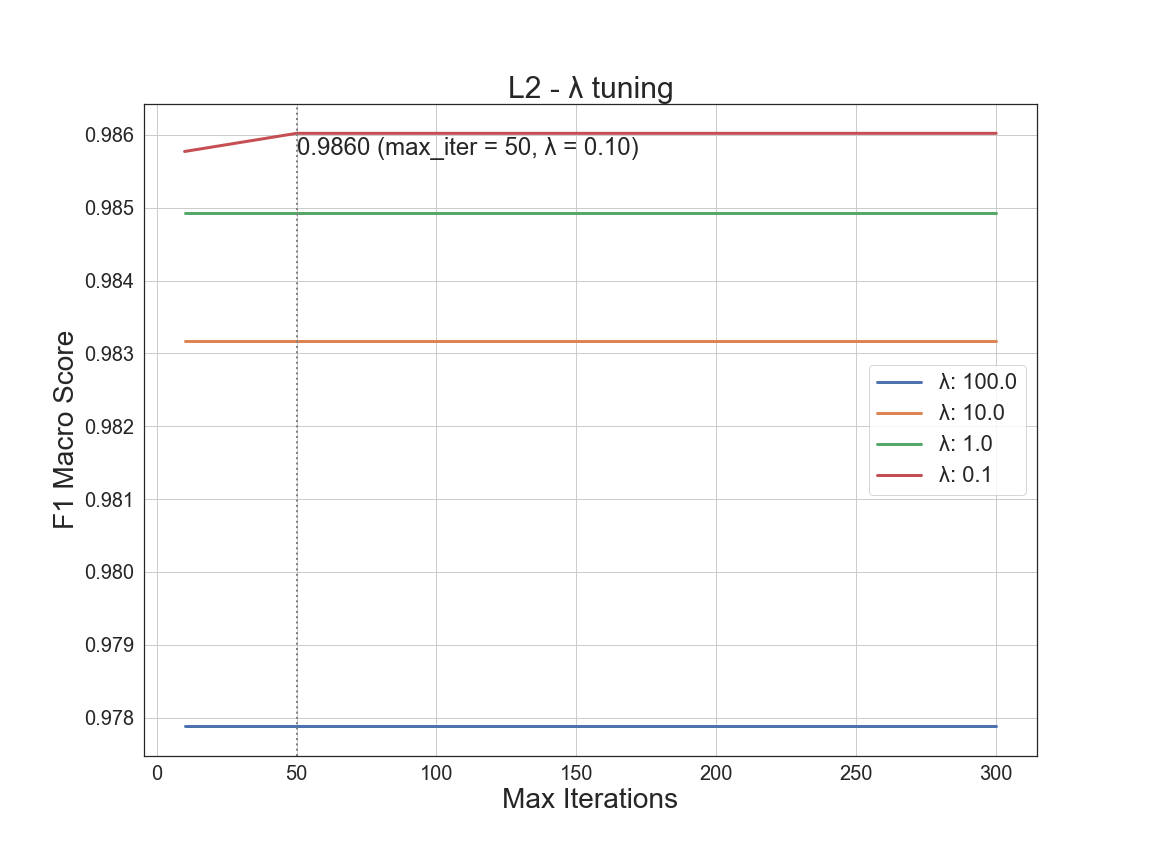
\includegraphics[width=\columnwidth]{chapter5/figure/logreg_l2_lambda.png}}\par 
	\caption{Regularization coefficient tuning}
\end{figure}

Figure \ref{fig:lr_lasso_lambda} highlights the slightly better results obtained with the Lasso penalty, with unitary $ \lambda $ coefficient (Lasso F1 score: 0.973).
As Figure \ref{fig:lr_ridge_lambda} shows, the ridge penalty needs to be weakened ($ \lambda $ = 0.1) in order to get close to the Lasso performance, which is a compromise hard to deal with. The smaller is the regularization coefficient, the higher is the model complexity, as said before.
Moreover, we decided to gather further consideration, by looking inside the weighting applied by those two terms.
Since we didn't have a lot of data for the training, we wanted to keep the regularization high enough to not fit the noise in the model.

We took a look inside the weighting performed by the model, with both L\textsubscript{1} and L\textsubscript{2} regularizations, in order to catch some insight from them.
The weights are composed by four vectors of twelve elements each: each vector represent the weights applied for a One-vs-Rest target classification, and each element of the vectors are mark the features the model has been fitted on. As said before, each of the three groups of four features represents the probabilities, for a sample, of membership to the classes.
In order to give a good representation, we considered just one vector of twelve elements, computed by averaging all the weights applied in all the OvR predictions.

\begin{center}
	\begin{tabular}{@{}cccc@{}}
		\multicolumn{4}{c}{Ridge regularization}\\
		\hline\hline
		\multicolumn{4}{c}{\textbf{KNN mean weights}}\\
		\hline
		\multicolumn{1}{c|}{\textit{NSFW}}&
		\multicolumn{1}{c|}{\textit{NS}}&
		\multicolumn{1}{c|}{\textit{SB}}&
		\multicolumn{1}{c}{\textit{FF}}\\
		\hline
		\multicolumn{1}{c|}{$ 3.4e^{-16} $}&
		\multicolumn{1}{c|}{$ 1.7e^{-15} $}&
		\multicolumn{1}{c|}{$ 3.2e^{-15} $}&
		\multicolumn{1}{c}{$ -1.1e^{-14} $}\\
		\hline
		\multicolumn{4}{c}{\textbf{Naive Bayes mean weights}}\\
		\hline
		\multicolumn{1}{c|}{\textit{NSFW}}&
		\multicolumn{1}{c|}{\textit{NS}}&
		\multicolumn{1}{c|}{\textit{SB}}&
		\multicolumn{1}{c}{\textit{FF}}\\
		\hline
		\multicolumn{1}{c|}{$ 2.8e^{-15} $}&
		\multicolumn{1}{c|}{$ -1.1e^{-14} $}&
		\multicolumn{1}{c|}{$ 9.8e^{-15} $}&
		\multicolumn{1}{c}{$ 4.8e^{-15} $}\\
		\hline
		\multicolumn{4}{c}{\textbf{Random Forest mean weights}}\\
		\hline
		\multicolumn{1}{c|}{\textit{NSFW}}&
		\multicolumn{1}{c|}{\textit{NS}}&
		\multicolumn{1}{c|}{\textit{SB}}&
		\multicolumn{1}{c}{\textit{FF}}\\
		\hline
		\multicolumn{1}{c|}{$ 8.7e^{-15} $}&
		\multicolumn{1}{c|}{$ -8.3e^{-15} $}&
		\multicolumn{1}{c|}{$ 1.0e^{-14} $}&
		\multicolumn{1}{c}{$ -1.7e^{-14} $}\\
		\hline\hline\\
	\end{tabular}
\end{center}
The Ridge regularization leads to very small weights, and negative ones too. Even with unitary $ \lambda  $ coefficient, it is hard to distinguish a discrimination among features. This approach would have yielded a smoother model, but with the ability to give a chance to every classifier to distinguish among targets.
We wanted to get some further insights from the other weighting.

\begin{center}
	\begin{tabular}{@{}cccc@{}}
		\multicolumn{4}{c}{Lasso regularization}\\
		\hline\hline
		\multicolumn{4}{c}{\textbf{KNN mean weights}}\\
		\hline
		\multicolumn{1}{c|}{\textit{NSFW}}&
		\multicolumn{1}{c|}{\textit{NS}}&
		\multicolumn{1}{c|}{\textit{SB}}&
		\multicolumn{1}{c}{\textit{FF}}\\
		\hline
		\multicolumn{1}{c|}{$ -0.660 $}&
		\multicolumn{1}{c|}{$ -0.185 $}&
		\multicolumn{1}{c|}{$ -0.465 $}&
		\multicolumn{1}{c}{$ -0.830 $}\\
		\hline
		\multicolumn{4}{c}{\textbf{Naive Bayes mean weights}}\\
		\hline
		\multicolumn{1}{c|}{\textit{NSFW}}&
		\multicolumn{1}{c|}{\textit{NS}}&
		\multicolumn{1}{c|}{\textit{SB}}&
		\multicolumn{1}{c}{\textit{FF}}\\
		\hline
		\multicolumn{1}{c|}{$ 0.578 $}&
		\multicolumn{1}{c|}{$ -0.054 $}&
		\multicolumn{1}{c|}{$ 0.072 $}&
		\multicolumn{1}{c}{$ 0.0 $}\\
		\hline
		\multicolumn{4}{c}{\textbf{Random Forest mean weights}}\\
		\hline
		\multicolumn{1}{c|}{\textit{NSFW}}&
		\multicolumn{1}{c|}{\textit{NS}}&
		\multicolumn{1}{c|}{\textit{SB}}&
		\multicolumn{1}{c}{\textit{FF}}\\
		\hline
		\multicolumn{1}{c|}{$ 1.993 $}&
		\multicolumn{1}{c|}{$ 2.147 $}&
		\multicolumn{1}{c|}{$ 2.049 $}&
		\multicolumn{1}{c}{$ 2.571 $}\\
		\hline\hline\\
	\end{tabular}
\end{center}
The L\textsubscript{1} term, as expected cut out some features from the model.
Looking at the excluded attributes, we noticed that the regularization caught the strenghts and the weaknesses of the classifiers. The text-based Naive Bayes classifier seemed to be useless when it came to detect Fake-Followers. It seemed legit, as the dictionary used by that category is the smallest and the most heterogeneus (lots of non english words are involved) in our dataset.
Lasso seemed to understand this behaviour and decided to not consider the opinion of that classifier, when it has to give its opinion about that bot cateogry.
Another insight got from L\textsubscript{1} is coming again from the Naive Bayes algorithm. The model couldn't distinguish with certainty Spam-Bots, since they act in a similar way, with respect to NSFW accounts. They just tweets click-baiting links, with catchy captions. A ``blind`` classifier struggles in understand the nature of those links. This is the reason that the contributes of the tex-based model had been almost discarded from the stacking meta-classifier.

\begin{figure}[htp!]
	\centering 
	\subfigure[Up to 150 iterations]{
		\label{fig:lr_lasso_close}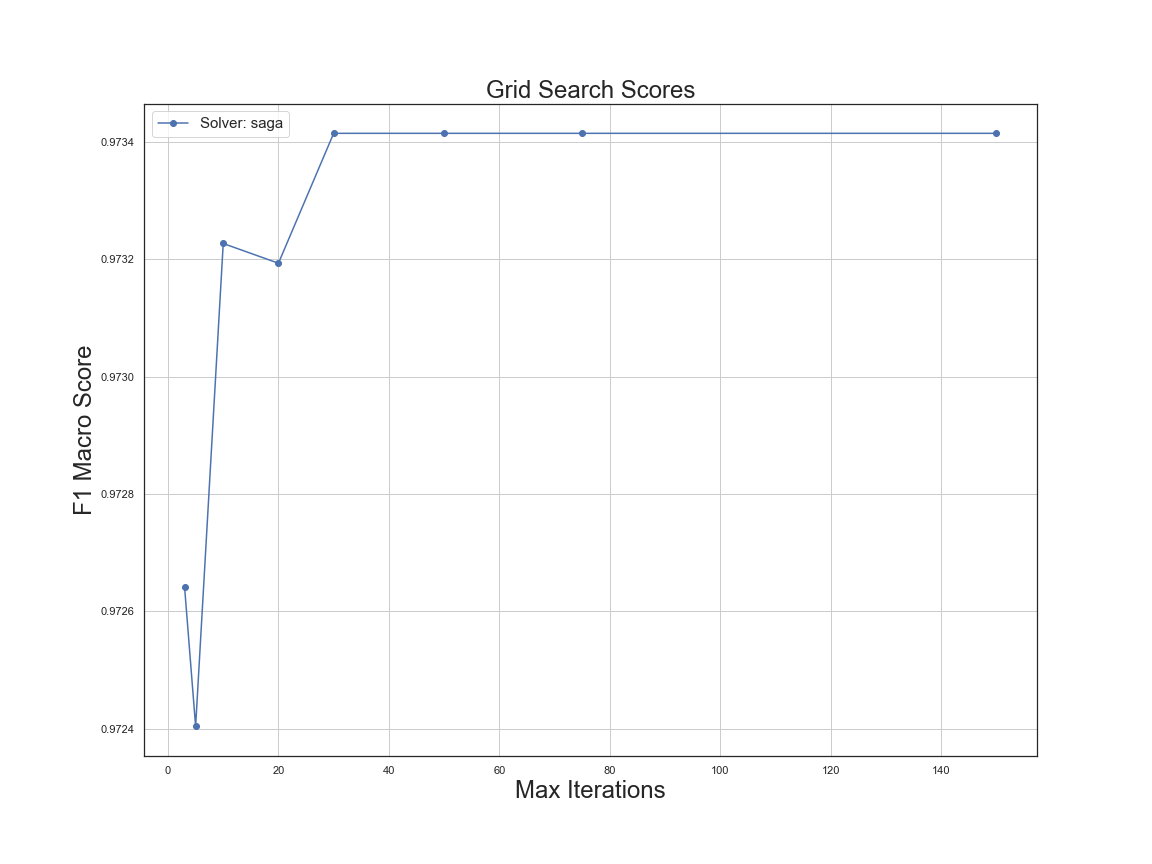
\includegraphics[width=\columnwidth]{chapter5/figure/logreg_l1_close.png}}
	\subfigure[Up to 5000 iterations - close-up view]{
		\label{fig:lr_lasso_far}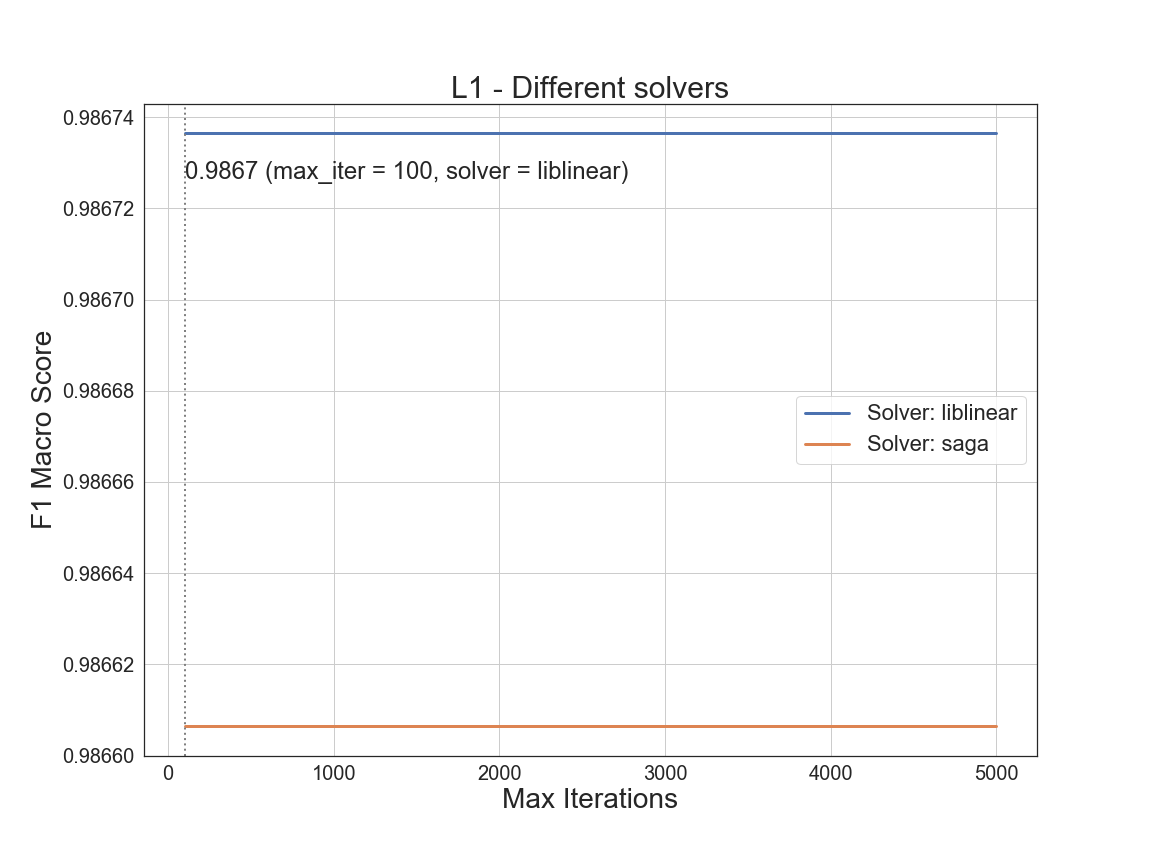
\includegraphics[width=\columnwidth]{chapter5/figure/logreg_l1_far.png}}
	\caption{Lasso Logistic Regression scores over solvers}
\end{figure}


Since we knew our dataset and we were aware of the bias it might contain, we preferred a lighter and sparser model, over a more complex one, even when the F1 scores used to match. We wanted our model to infer on new unseen data and to be ready to give a representative statistical description of the actual situation on Twitter.
We had to be far-sighted and not to recline on the accomplishments of the 10-fold crossvalidation. We thought that the Lasso model would have been performing better in out-of-box predictions.

We kept the L\textsubscript{1} penalty, with $ \lambda  = 1 $   and proceeded with the hyperparameters tuning.

Figure \ref{fig:lr_lasso_close} shows the trend in the F1 score, along with the increasing number of iterations, applying the \textit{SAGA} \cite{SAGA} solver (a variant of the \textit{Stochastic Average Gradient} \cite{SAG} optimization that supports Lasso penalty) and the \textit{LIBLINEAR} \cite{Liblinear}, an open source library for large-scale linear classification.

As it can be seen in Figures \ref{fig:lr_lasso_far}, by increasing the number of maximum iterations, up to 5000, the performances remain stable with every solver.
The algorithms seem to not improve after 75 maximum iterations setted.
Moreover, the LIBLINEAR solver gains slightly better results, in terms of F1 score, as it reaches 0.9867 in this metric, compared with the score obtained with LIBLINEAR solver, which is 0.9867.

The final Logistic Regression meta-classifier has been fitted with the Scikit-learn library, with this setting:\\
\textit{LogisticRegression(max\_iter = 100, penalty = ``l1``, solver = ``liblinear``, C = 1, multi\_class = ``multinomial``, fit\_intercept = True)}.\\
The \textit{C} parameter stands for $ \frac{1}{\lambda} $, the regularization coefficient.
This setting obtained the following scores in a 10-fold crossvalidation:
\begin{itemize}
	\item[\PencilRight] \textit{Precision}: \textbf{0.987}
	\item[\PencilRight] \textit{Recall}: \textbf{0.986}
	\item[\PencilRight] \textit{F1 score}: \textbf{0.987}
\end{itemize}

The stacking ensemble performance is resumed in Figure \ref{fig:stacking_performance}, where all the components are first measured individually to show that the combination of them improves the overall F1 score.
\begin{figure}[htp!]
	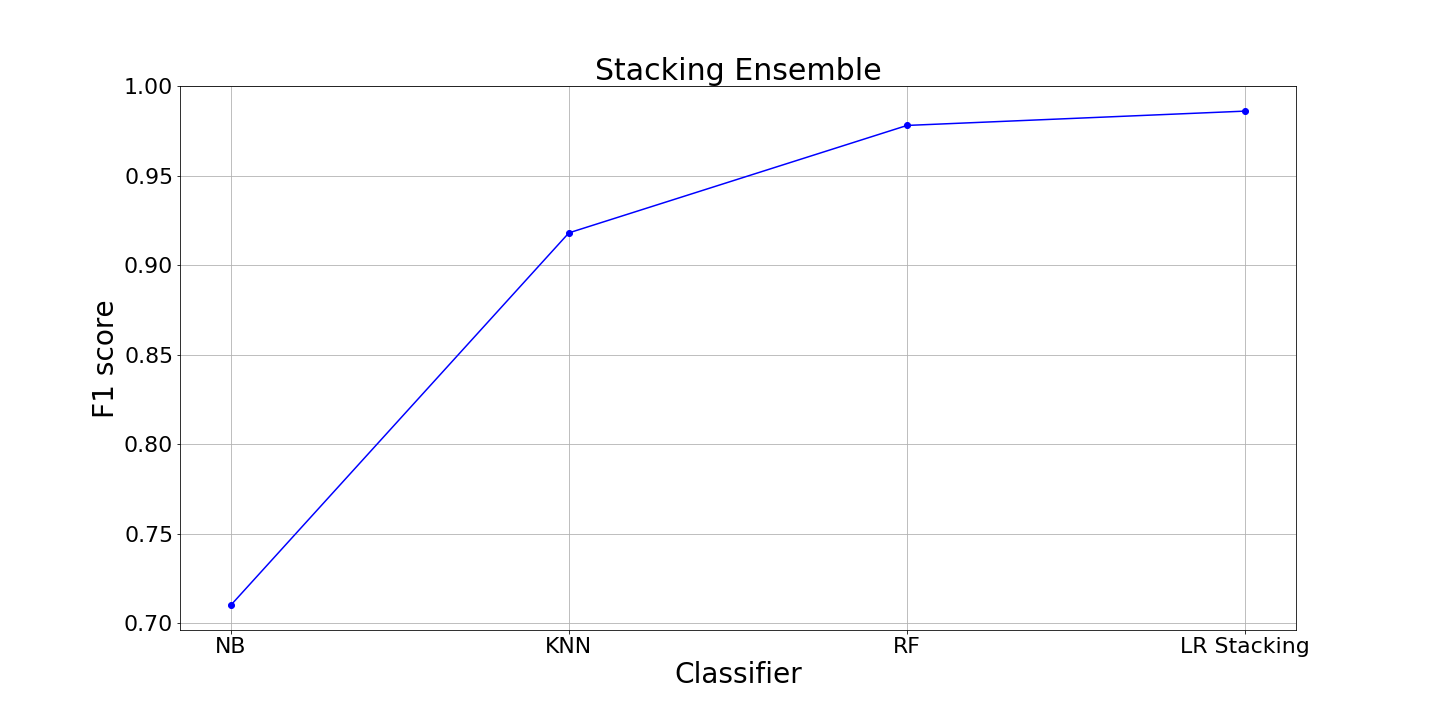
\includegraphics[width=\columnwidth]{chapter6/figure/stacking_performance.png}
	\caption{Stacking ensemble performance}
	\label{fig:stacking_performance}
\end{figure}

\section{Prediction pipeline}
\label{predicion_pipeline}
The final model is represented by an execution pipeline, involving a first binary classifier and then a mutli-class ensemble.

As described by figure \ref{fig:prediction_pipeline}, In order to perform a prediction over a new sample the process is the following:
\begin{enumerate}
	\item User and tweets data retrieving with Twitter APIs
	\item Prepare data with binary extrinsic features and strip image attributes, in order to output binary probability prediction (\textbf{Binary Random Forest})
	\item Prepare data and perform features computation to output multi-class probability prediction (\textbf{All-features multi-class Random Forest})
	\item Strip all attributes, except for the user features, weight them with Information Gain-driven proportions to output multi-class probability prediction (\textbf{User-based multi-class KNN})
	\item Prepare and treat text to perform text-based probability prediction (\textbf{Text-based multi-class Naive Bayes})
	\item Build new features vector with the stacked outcomes of the mutliclass classifiers
	\item Compute the final mutliclass probabilistic prediction with the meta-classifier (\textbf{Multinomial Logistic Regression})
	\item Use the multi-class division to repartition the bot probability provided by the binary model
\end{enumerate}
The binary classifier returns two values: the membership probability for the bot category and the one for the genuine class.
The percentage that marks the bot nature of the examined account gets partitioned by the outcome of the multi-class stacking ensemble.
The pipeline will be performed by a web application, in order to provide a useful classification tool for every internet user.

\begin{figure}[t!]
	\begin{center}
		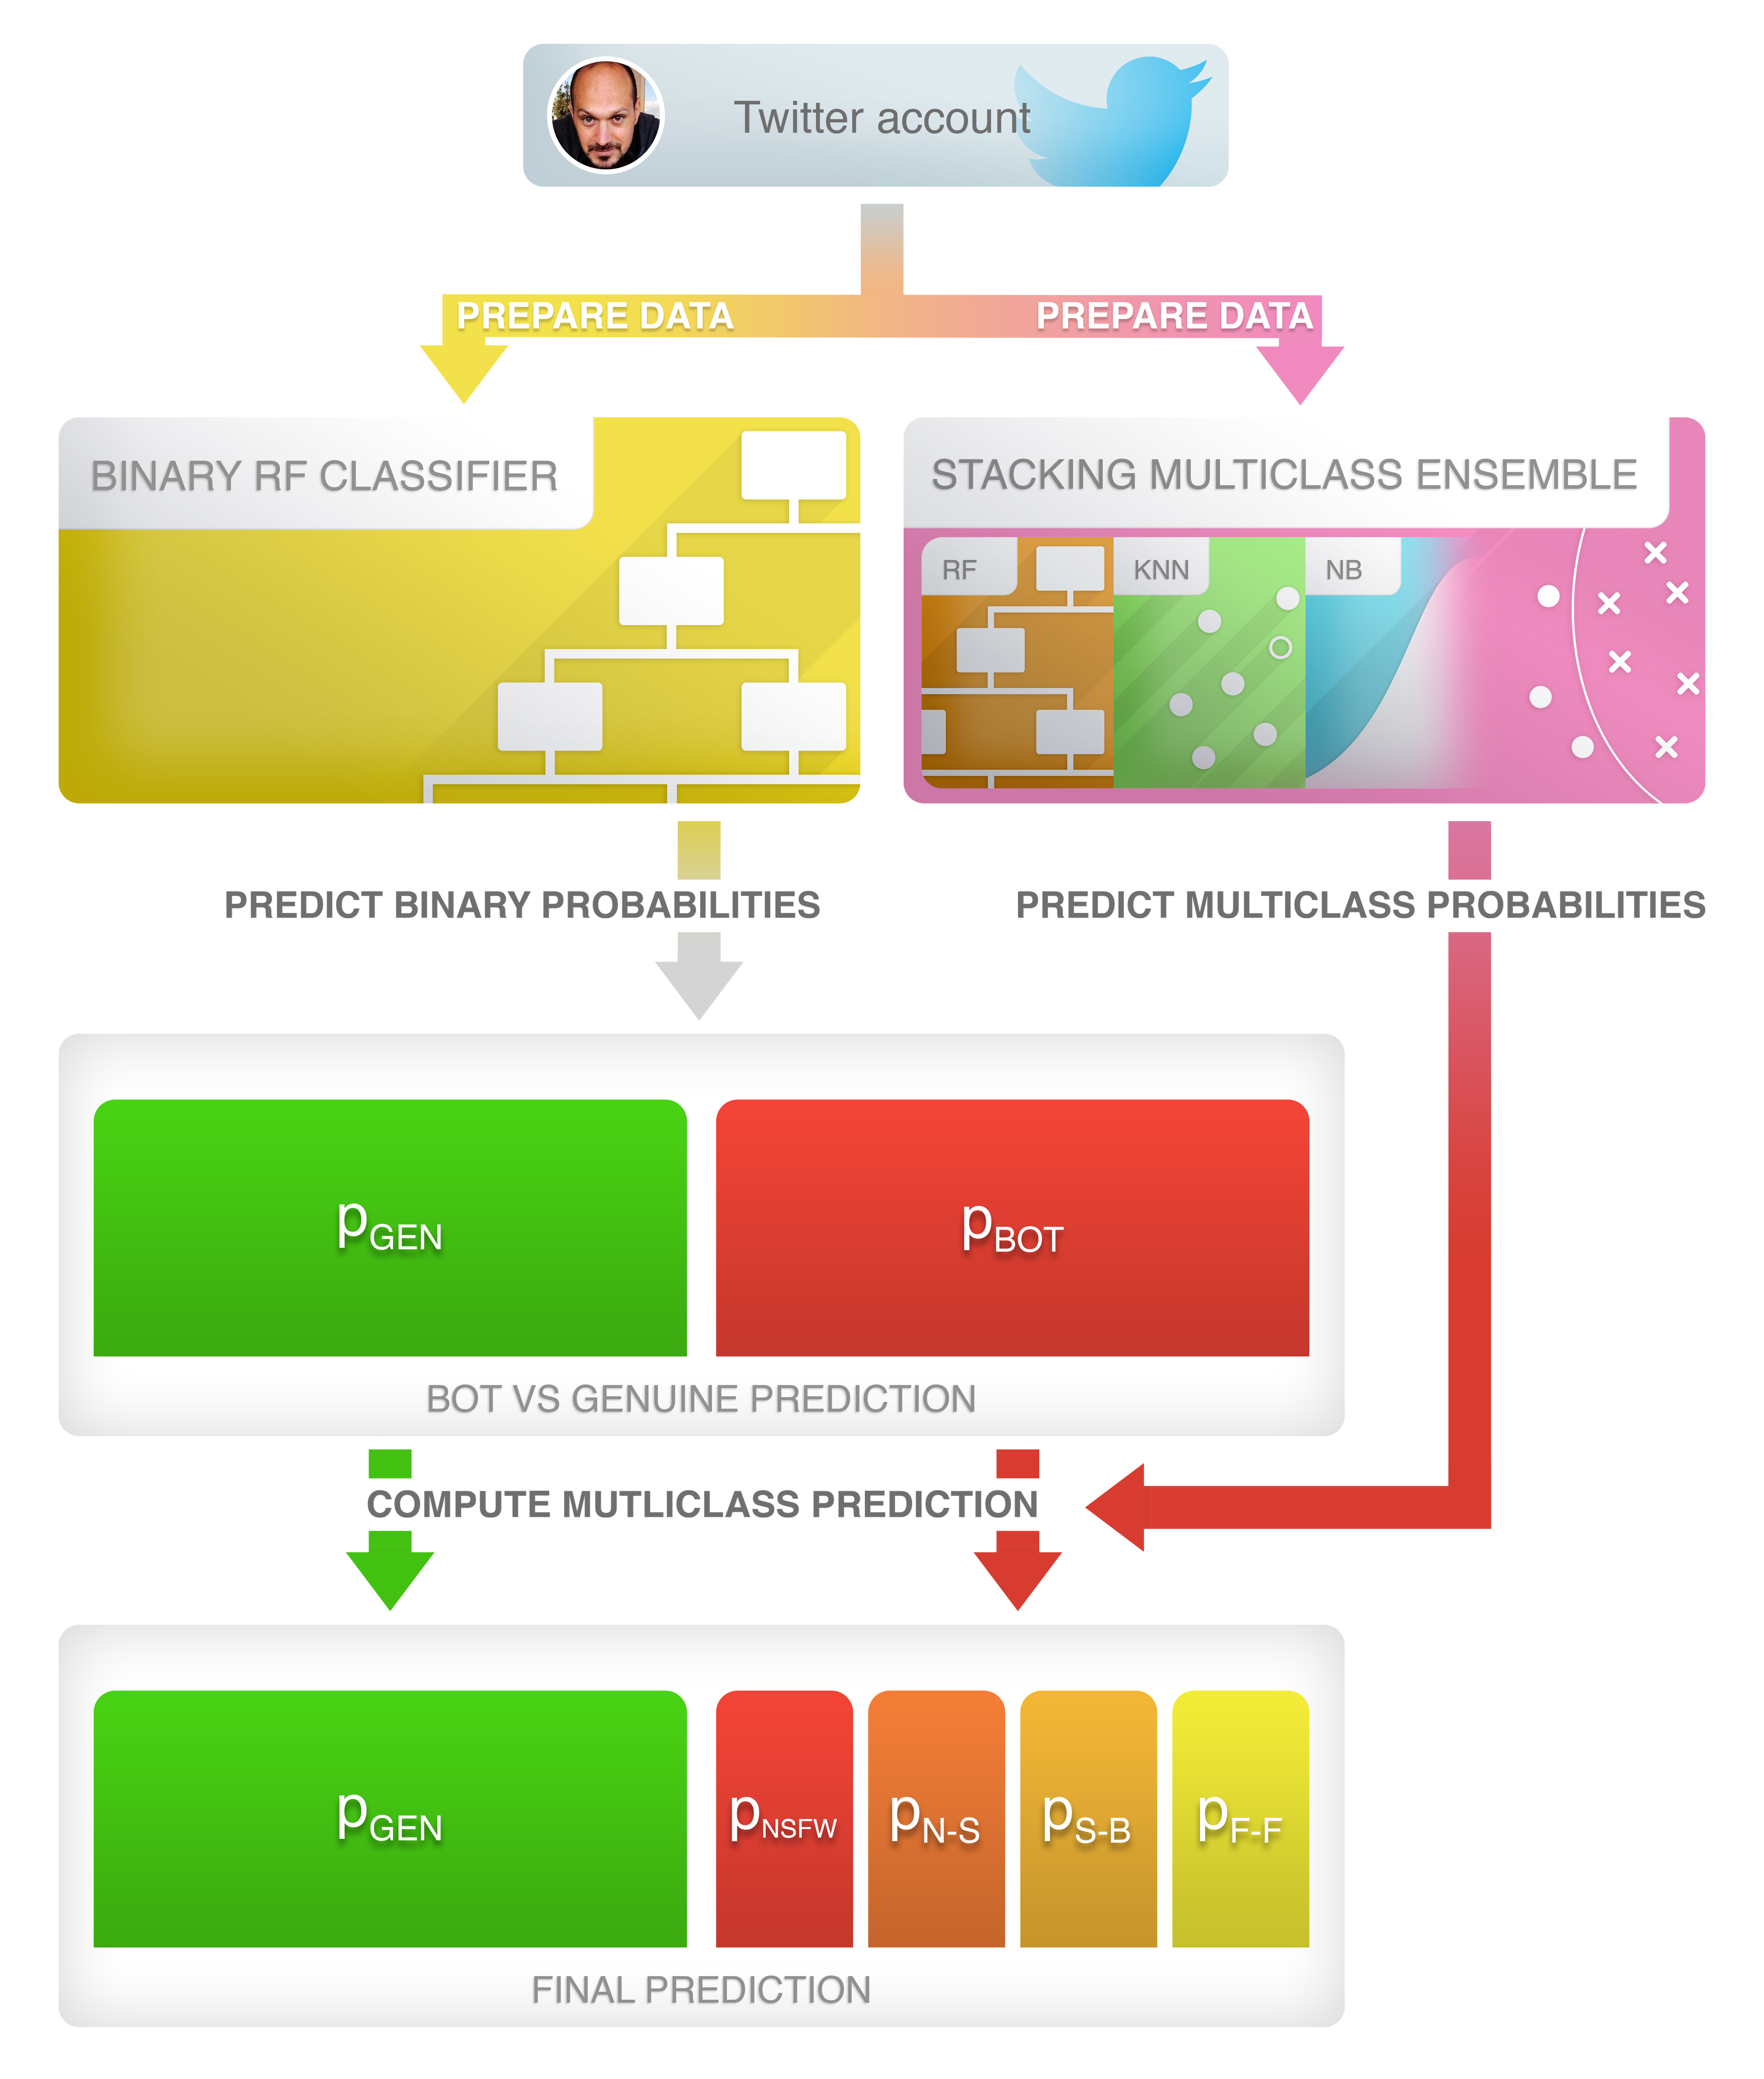
\includegraphics[width=\columnwidth]{chapter5/figure/pred_pipeline.png}
	\end{center}
	\caption{Final prediction pipeline}
	\label{fig:prediction_pipeline}
\end{figure}